\section{Experiment Design and Methodology}\label{section:Experiment_Design_and_Methodology}
\textbf{Research Design:} Overview of the experimental framework.\newline
\textbf{Methodology:} Detailed description of the methods used for data collection and analysis.\newline
\textbf{Variables:} Identification of key variables and how they are measured.\newline
\textbf{Procedures:} Step-by-step outline of the experimental process.\newline

Each of the participants were asked to produce 25 10-item sequences, each of which was composed of 10 ones or zeros (representing heads or tails).

\subsection{Introduction}
As discussed in Chapter~\ref{production_of_random_binary_sequences}, the experimental design used in this project closely aligns with that which was established by Nickerson and Butler~\cite{nickerson:2009}, serving as the foundational basis for the procedures used in this experiment. By adapting their established methodology to this novel application, this project extends the findings of their work by not only comparing the subjects' generated sequences with those that would be expected of a random process according to the statistical definition but also by testing the predictability of each subject's current response according to their previous responses using Prediction with Expert Advice and Vovk's Aggregating Algorithm~\cite{vovk:1990} since, in theory, the more random a subject's generated sequence are, the less predictable their responses and the greater the loss incurred by both the Learner and each of the Experts in the Aggregating Algorithm.

\subsection{Experimental Design}
In this chapter, we will outline the experimental design of this study, which aims to explore how well individuals can generate random binary sequences when compared to the theoretical definition of randomness and what they have previously inputted. 

The subjects of this study were typically students of Royal Holloway, University of London. They were tasked with generating several 10-item random binary sequences by typing them into the web application hosted on \href{https://arbarraclough.github.io/aggregating_algorithm/}{GitHub Pages}. Each of these sequences comprised $10$ $0$s or $1$s (representing Heads and Tails) in whatever order the subject saw fit and at their own pace. Before typing their sequences, the subjects were prompted with the following message on a modal screen shown upon loading the site:

\begin{quote}
    \textit{Your task is to create a table of sequences each consisting of 10 items, either 0 or 1.}
    
    \textit{Imagine that several people have each tossed a fair coin 10 times and the results of their tosses are recorded in a table, with each row recording the outcomes of the 10 tosses by one person.}
    
    \textit{Your goal is to produce this table in such a way that if compared with a table of the results of actual coin tosses, it would not be possible to distinguish which table represented the actual coin tosses with statistical tests and which didn't.}
\end{quote}

Unlike in Nickerson and Butler's experiment where, as the subject typed in their sequence, it would remain on screen until the entire 10-item sequence was completed before disappearing and the next 10-item sequence could be entered, the subject's ``sequences'' in this experiment would be treated as one concatenated sequence for the sake of the Aggregating Algorithm and would be displayed as such in a table on screen (shown in Figure 3).

\begin{figure}[h]
\centering
    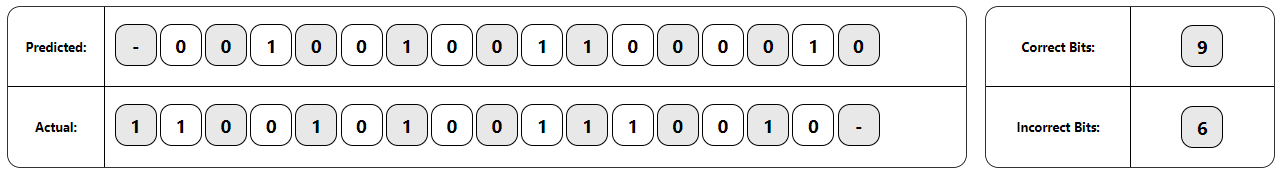
\includegraphics[width=0.9\textwidth]{images/sequence_input.png}
    \caption{Inputted Sequence Displayed in the Web Application}
\end{figure}

This is because that short of a time horizon—10 time steps—would be insufficient to allow the Aggregating Algorithm to identify patterns in the user's inputs and determine which experts should have higher weighting, resulting in poorer predictions by the Learner. However, while there is this distinction in how the sequences are treated, how they are fed back to the user follows \cite{nickerson:2009} in that the concatenated sequence is chunked into groups of 10 when applicable and shown to the user in a separate table (shown in Figure 4). This is because, as discussed in Chapter~\ref{production_of_random_binary_sequences}, the human short-term memory roughly spans 7 (+/- 2) items and by chunking subsequences, the subject can quickly see what they have previously input beyond that span and continue to type inputs that they feel are random.

\begin{figure}[h]
\centering
    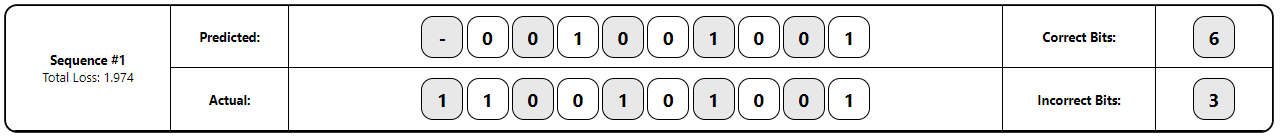
\includegraphics[width=0.9\textwidth]{images/past_sequences.png}
    \caption{Past Sequences Displayed in the Web Application.}
\end{figure}

Given this foundation, we can now discuss how the Aggregating Algorithm for Specialist Experts (AASE) was applied to this experiment. As hinted at in Chapter 2, the primary focus of this dissertation is the Discrete Binary Game defined as $\langle \Gamma, \Omega, \lambda \rangle$ where $\Gamma = [0, 1]$, $\Omega = \{ 0, 1 \}$, and $\lambda = \lambda_{\text{SQ}}(\gamma_t, \omega_t) = (\gamma_t - \omega_t)^2$.

\subsection{Procedure}
Testing
\newpage